\documentclass[background.tex]{subfiles}

\begin{document}
\subsection{Cauder}
In questa sottosezione introduco Cauder ovvero: 
	\begin{enumerate}
		\item La sintassi che supporta, ponendo enfasi sulle funzioni rilevanti per questa tesi.
		\item Le strutture dati che manipola.
		\item La sua semantica e come modifica le strutture dati.
	\end{enumerate}
Per tutta questa sottosezione faccio riferimento a \cite{lanese19}.\\
\textbf{1) La sintassi supportata:}\\
La sintassi del linguaggio può essere trovata nella Figura \ref{fig2}. Un modulo è una sequenza di definizioni di funzioni, dove ogni nome di funzione f / n (atom / arity) ha una definizione associata della forma $\displaystyle fun (X_{1},..., X_{n}) \xrightarrow{body} e$.
Il corpo di una funzione è \underline{un'espressione}, che può includere variabili, letterali, nomi di funzioni, liste, tuple, chiamate a funzioni predefinite, principalmente operatori aritmetici e relazionali, applicazioni di funzioni, espressioni case, associazioni let e espressioni di ricezione; inoltre, consideriamo anche le funzioni \textit{spawn}, \textit{"!"} (per inviare un messaggio) e \textit{self()} (ritorna il pid del processo chiamante) che in realtà sono incorporate nel linguaggio Erlang.
\begin{figure}[!ht]
  $\displaystyle
  \begin{array}{rcl@{~~~~~~}l}
    \mathit{module} & ::= & \mathsf{module} ~ Atom = %%[fname_1,\ldots,fname_n] =
    \mathit{fun}_1,\ldots,\mathit{fun}_n\\
    {\mathit{fun}} & ::= & \mathit{fname} = \mathsf{fun}~(X_1,\ldots,X_n) \to expr \\
    {\mathit{fname}} & ::= & Atom/Integer \\
    lit & ::= & Atom \mid Integer \mid Float \mid \nil \\
    expr & ::= & \mathit{Var} \mid lit \mid \mathit{fname} \mid [expr_1|expr_2]
                 \mid   \{expr_1,\ldots,expr_n\} \\
    & \mid & \mathsf{call}~expr~(expr_1,\ldots,expr_n) 
    \mid \mathsf{apply}~expr~(expr_1,\ldots,expr_n) \\
    & \mid &
    \mathsf{case}~expr~\mathsf{of}~clause_1;\ldots;clause_m~\mathsf{end}\\
    & \mid & \mathsf{let}~\mathit{Var}=expr_1~\mathsf{in}~expr_2 
    \mid \mathsf{receive}~clause_1;\ldots;clause_n~\mathsf{end}\\
    & \mid & \mathsf{spawn}(expr,[expr_1,\ldots,expr_n])  
     \mid expr_1 \:!\: expr_2 \mid \mathsf{self}()\\
    clause & ::= & pat ~\mathsf{when}~expr_1 \to expr_2
    \\
    pat & ::= & \mathit{Var} \mid lit \mid [pat_1|pat_2] \mid
    \{pat_1,\ldots,pat_n\} \\
  \end{array}
  $
\caption{Regole sintattiche del linguaggio} 
\label{fig2}
\end{figure}
Di seguito spiego con maggior dettaglio solo alcune \textit{expressioni}.
Il motivo di ciò risiede nel fatto che l'estensione di Cauder risulta mostrare analogie, più o meno rilevanti, con queste regole sintattiche e le loro regole semantiche.\\
\begin{itemize}
	\item $\displaystyle \mathsf{spawn}(expr,[expr_{1},...,expr_{n}])\xrightarrow{return}SpawnedPid$: La chiamata alla funzione $\mathsf{spawn}$ crea un nuovo processo, che inizia con la valutazione di $\displaystyle \mathsf{apply}(expr,[expr_{1},...,expr_{n}])$. Ritorna il \textit{pid} del processo appena generato.
	\item $\displaystyle expr_{1}~!~expr_{2}\xrightarrow{return}expr_{2}$: La chiamata alla funzione send (!) invia il messaggio \textit{expr2} al processo con \textit{pid $expr_{1}$}. Ritorna il messaggio inviato ovvero \textit{$expr_{2}$}.
	\item $\displaystyle \mathsf{receive}~clause_{1};...;clause_{n}\xrightarrow{return}expr_{2}$ di clause matching: L'espressione $\mathsf{receive}$ attraversa i messaggi nella coda dei messaggi del processo finché uno di essi non corrisponde a un ramo nell'istruzione di ricezione; dovrebbe trovare il primo messaggio v nella coda tale che $\exists$ clause $\in$ \{$clause_{1}$;...;$clause_{n}$\} tale che v matcha \textit{pat} di clause $\wedge$ \textit{$expr_{1}$} di clause==$\mathsf{true}$; ritorna \textit{$expr_{2}$} di clause, con l'ulteriore effetto collaterale di eliminare il messaggio v dalla coda dei messaggi del processo. Se non sono presenti messaggi corrispondenti nella coda, il processo sospende la sua esecuzione finché non arriva un messaggio corrispondente.
\end{itemize}
Nel punto relativo alla semantica ometto la spiegazione della receive, in quanto è interessante solo dal punto di vista comportamentale.\\
\textbf{2) Le strutture dati di Cauder:}\\
In questa sezione vado a definire le strutture dati gestite da Cauder.
Nella figura \ref{fig3} sottostante mostro come lo stato di Cauder viene rappresentato graficamente.
Ad ogni struttura dati che introduco, associerò come essa viene rappresentata internamente in Cauder e come venga rappresentata graficamente, facendo riferimento alla figura sopracitata.
\begin{figure}[!ht]
	\centerline{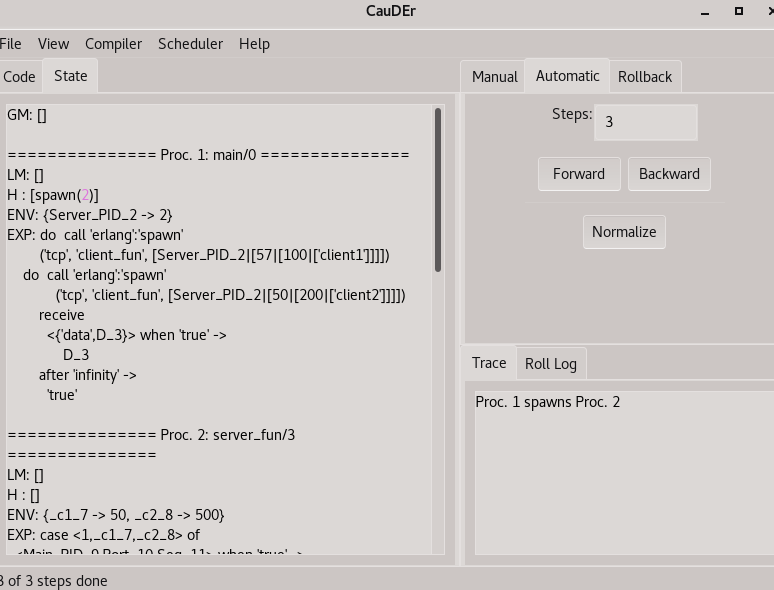
\includegraphics[scale=0.5]{./Background/Cauder/Imgs/CauderStato}}
	\caption{Lo stato di Cauder.}
	\label{fig3}
\end{figure}
Un \textit{sistema} in esecuzione viene denotato tramite $\Gamma$;$\Pi$, dove $\Gamma$ denota la mailbox global ovvero \underline{l'insieme} dei \textit{messaggi inviati} in attesa di essere consegnati, mentre $\Pi$ denota \underline{l'insieme} dei \textit{processi} nel sistema.
In Cauder le varie strutture verranno implementate tramite i \textit{record} \cite{erlangRecord}.
Il \textit{sistema} viene implementato in Cauder tramite un \textit{record sys} contenente i seguenti campi:
	\begin{itemize}
		\item \textit{\textbf{sched}}: denota la tipologia di scheduling delle azioni da utilizzare. Cauder utilizza due politiche di scheduling:
			\begin{itemize}
				\item RANDOM: L'azione viene scelta casualmente \textit{tra tutte le azioni possibili} del sistema.
				\item PRIO\_RANDOM: L'azione viene scelta casualmente \textit{tra tutte le azioni effettuabili dai processi} e se non ce ne sono viene scelta casualmente \textit{tra tutte le azioni effettuabili per la schedulazione dei messaggi}.
			\end{itemize}
			Nel punto della semantica verrà spiegato il perchè è necessaria una schedulazione dei messaggi.
		\item \textit{\textbf{msgs}}: denota la mailbox globale ovvero $\Gamma$. Nella figura \ref{fig3} viene rappresentata da \textit{GM}.
		\item \textit{\textbf{procs}}: denota l'insieme dei processi ovvero $\Pi$. Nella figura \ref{fig3} viene rappresentata dalla lista \textit{======Proc.N:fun/M====}.
		\item \textit{\textbf{trace}}: denota le azioni effettuate nel sistema. Nella figura \ref{fig3} vengono visualizzate nel \textit{tab Trace}.
		\item \textit{\textbf{roll}}: denota le operazioni di \textit{roll} effettuate nel sistema. Nella figura \ref{fig3} vengono visualizzare nel \textit{tab Roll log}.
	\end{itemize}
Illustrato la struttura di un \textit{sistema} mi soffermo sui campi \textit{msgs} e \textit{procs}, in quanto, \textbf{per motivi diversi e che verrano spiegato nella sezione relativa all'estensione}, risultano essere rilevanti per questa tesi.
Il campo \textit{sched} verrà menzionato nella parte dell'estensione, ma non approfondito in quanto non troppo rilevante per questa tesi.
\textit{Msgs} risulta essere implementata tramite una \textit{lista} di \textit{msg}.\\
Formalmente \textit{msg} è una tripla del tipo \textit{(pid\_dest,value,time)}. Il campo \textit{time} risulta essere necessario in quanto discrimina quel messagio specifico, dato che potrei avere più messaggi con lo stesso valore e destinatario.
Banalmente, un \textit{msg} viene implementato tramite un \textit{record msg} contenente i campi sopra citati.
Analogalmente a \textit{msgs}, \textit{procs} viene implementato tramite una \textit{lista} di \textit{proc}.
Formalmente \textit{proc} viene denotato tramite \textit{$\langle$ p,$\theta$,e,h,lm$\rangle$}, dove:
	\begin{itemize}
		\item \textit{p}: rappresenta il pid del processo.
		\item \textit{$\theta$}: rappresenta l'ambiente del processo, ovvero \textit{l'insieme} dei bindings.
		\item \textit{e}: rappresenta l'espressione da valutare.
		\item \textit{h}: rappresenta \textit{l'history} del processo, ovvero la \textit{sequenza} di tutte le azioni che il processo ha effettuato.
		\item \textit{lm}: rappresenta la mailbox del processo, ovvero la \textit{sequenza} di tutti i messaggi \textit{schedulati} il cui destinatario è il processo.
	\end{itemize}
\textit{Proc} viene implementata tramite un \textit{record proc} con i seguenti campi e farò riferimento alla figura \ref{fig3} per le visualizzazioni:
	\begin{itemize}
		\item \textit{pid}: implementa \textit{p} ed è visualizzato tramite \textit{N} in\\ \textit{======Proc.N:fun/M====}.
		\item \textit{hist}: implementa \textit{h} ed è visualizzato tramite \textit{H}.
		\item \textit{env}: implementa \textit{$\theta$} ed è visualizzato tramite \textit{ENV}.
		\item \textit{exp}: implementa \textit{e} ed è visualizzato tramite \textit{EXP}.
		\item \textit{mail}: implementa \textit{lm} ed è visualizzato tramite \textit{LM}.
	\end{itemize}
	Il \textit{record proc} possiede campi aggiuntivi ma che non menziono dato la non rilevanza per questa tesi.\\
\textbf{2) La semantica di Cauder:}\\
In questo punto introduco la semantica di Cauder. Più precisamente mostro solo un sottoinsieme di queste regole, in quanto le altre non sono rilevanti per questa tesi.
Evidenzio \textbf{3} regole, che vado ad illustrare, lavorando su un processo generico P \textit{che esegue la regola descritta}, ovvero $\displaystyle \langle p,\theta,e,h,lm\}$ e su un sistema generico S, ovvero $\Gamma$;$\Pi$.\\
Essendo un linguaggio funzionale ad ogni passo creo delle nuove strutture dati sulla base delle vecchie, costruendo nuovi stati a partire dai precedenti.\\
Come già accennato in precedenza, sia gli insiemi che le sequenze vengono implementati come \textit{liste}. A livello implementativo, per l'aggiunta di un elemento in una lista, uso la notazione [H$\mid$L], ovvero creo una nuova lista aggiungendo \textit{H} in testa alla lista \textit{L}, mentre per l'eliminazione di un elemento H si verificano due casi:
	\begin{itemize}
		\item se H è in testa ([H$\mid$L]) prendo solo L.
		\item se H non è in testa uso un \textit{filter} sulla lista prendendo tutti gli elementi diversi da H.
	\end{itemize}
Nella spiegazione della semantica, per la modifica degli insiemi utilizzo la notazione insiemistica mentre per le sequenze utilizzo direttamente la notazione implementativa.
Ciò viene fatto per tenere evidenziato cosa è un insieme e cosa è una sequenza.
Denoto le costanti tramite $\mathsf{valore\_atomo}$, mentre per riferirmi ai campi delle strutture dati, utilizzo la notazione punto (esempio: flag di un processo P = P.f).\\
\textbf{Se non esplicitamente utilizzata, allora mi riferisco ai campi di un processo}.
Riguardo ai campi $\theta$ ed \textit{e} se non esplicitamente dichiarati, si intende la loro modifica secondo la loro gestione interna da parte di Cauder, poichè non rilevanti in quella specifica regola.
Nel punto 1 ho posto enfasi solo su 3 regole sintattiche, ovvero la $\mathsf{spawn}$ per generare processi, la $\mathsf{send}$ per inviare un messaggio e la $\mathsf{receive}$ per elaborare un messaggio presente nella local mailbox del processo.
\textbf{Ma non è definito come un messaggio venga recapitato dalla global mailbox alla local mailbox, dato l'asincronicità di Erlang detta nell'introduzione}. La quarta regola semantica che emerge (\textit{rule sched}) serve per simulare questa asincronicità.\\
\textbf{SEMANTICA IN AVANTI}:
\begin{itemize}
	\item \textit{\textbf{rule spawn}}: Informalmente questa regola va ad inserire in $\Pi$ un \textit{proc} con \textit{history} e \textit{local mailbox} vuote. Formalmente:\\
	Sia P'=$\displaystyle \langle p',\theta'=\empty,e'=\mathsf{apply}(fun(expr_{1}...expr_{n})),h'=[],lm=[]\rangle$ il processo spawnato.\\
	Sia h''=$\displaystyle [\{\mathsf{spawn},\theta,e,p'\} \mid h]$.\\
	Sia P''=$\displaystyle \langle p,\theta'',e'',h'',lm\rangle$.\\
	Il sistema risultante da questo passaggio sarà S'=$\displaystyle \Gamma;\Pi\setminus\{P\}\cup\{P',P''\}$.
	\item \textit{\textbf{rule send}}: Informalmente questa regola va ad inserire in $\Gamma$ un \textit{msg}. Formalmente:\\
	Sia msg=\textit{(dest\_pid,payload,time)}.\\
	Sia h'=$\displaystyle [\{\mathsf{send},\theta,e,msg\} \mid h]$.\\
	Sia P'=$\displaystyle \langle p,\theta',e'',h',lm \rangle$.
	Il sistema risultante da questo passaggio sarà S'=$\displaystyle \Gamma\cup\{msg\};\Pi\setminus\{P\}\cup\{P'\}$.
	\item \textit{\textbf{rule sched}}: 
	Sia msg=\textit{(dest\_pid,payload,time)} il messaggio selezionato per la schedulazione.
	Sia lm'=[msg $\mid$ lm].
	Sia P'=$\displaystyle \langle p,\theta,e,h,lm'\rangle$.\\
	Il sistema risultante da questo passaggio sarà S'=$\displaystyle \Gamma\setminus\{msg\};\Pi\setminus\{P\}\cup\{P'\}$.
\end{itemize}
\textbf{SEMANTICA ALL'INDIETRO}:
	\begin{itemize}
		\item \textit{\textbf{rule spawn}}: Informalmente questa regola va ad eliminare da $\Pi$ un \textit{proc} spawnato. Come precondizione per effettuare l'undo della $\mathsf{spawn}$, bisogna che il processo spawnato abbia \textit{history} e \textit{local mailbox} vuote. Più formalmente bisogna che P'=$\displaystyle \langle p',\theta',e',h'=[],lm=[]\rangle$. Se non fosse rispettata questa precondizione si rischierebbe di violare il Loop Lemma.
		Ipotizziamo di avere 3 processi cosi definiti, in cui il processo 1 spawna il secondo e il secondo spawna il terzo.
		Abbiamo una situazione del genere:
		\begin{enumerate}
			\item $\displaystyle \langle p',\theta',e',h',lm' \rangle$ con h'=$\displaystyle [\{\mathsf{spawn},\theta,e,p''\} \mid h_{1}]$.
			\item  $\displaystyle \langle p'',\theta'',e'',h'',lm''\rangle$ con h''=$\displaystyle[\{\mathsf{spawn},\theta,e,p'''\} \mid h_{2}]$.
			\item il terzo processo non è rilevante.
		\end{enumerate}
		Ora facciamo l'undo della $\mathsf{spawn}$ del secondo processo per poi rifarla.
		Ci ritroviamo nella seguente situazione:
			\begin{enumerate}
			\item $\displaystyle \langle p',\theta',e',h',lm' \rangle$ con h'=$\displaystyle [\{\mathsf{spawn},\theta,e,p''\} \mid h_{1}]$.
			\item $\displaystyle \langle p'',\theta'',e'',h'',lm'' \rangle$ con h''=[] ed lm''=[].
			\item il terzo processo non è rilevante.
		\end{enumerate}
		Abbiamo fatto l'undo di un'azione per poi rifarla e siamo finiti su uno stato diverso, violando il Loop Lemma.\\
		Posta vi sia questa condizione, l'undo di una spawn si formalizza così:
		Sia h=$\displaystyle [\{\mathsf{spawn},\theta,e,p'\} \mid h_{old}]$.\\
		Sia P' il processo con pid \textit{p'}.\\
		Sia P''=$\displaystyle \langle p,\theta'' = \theta,e''=e,h''=h_{old},lm \rangle$.\\
		Allora il sistema evolve in S'=$\displaystyle \Gamma;\Pi\setminus\{P',P\}\cup\{P''\}$.
		\item \textit{\textbf{rule send}}: Informalmente questa regola elimina un \textit{msg} da $\Gamma$. Come precondizione per effettuare l'undo di una $\mathsf{send}$, bisogna che il messaggio \textit{msg} sia presente in $\Gamma$. Se così non fosse si rischierebbe di violare il Loop Lemma.
		Ipotizziamo questo scenario:
		Un messaggio \textit{msg=(p',val,time)} è presente nella local mailbox di p' ( è già stato schedulato). Quindi ho questi due processi:
			\begin{itemize}
				\item P'=$\displaystyle \langle p',\theta',e',h',lm'\rangle$ con lm'=[msg  $\mid$ lm] che è il destinatario del messaggio.
				\item $\displaystyle \Gamma'=\Gamma\setminus\{msg\}$.
			\end{itemize}
		Se facessi l'undo della send per poi rifarla subito dopo mi ritroverei in questa situazione:
			\begin{itemize}
				\item P'=$\displaystyle \langle p',\theta',e',h',lm'\rangle$ con lm'=[msg  $\mid$ lm] che è il destinatario del messaggio.
				\item $\displaystyle \Gamma'=\Gamma\cup\{msg\}$.
			\end{itemize}
		In sostanza mi troverei con un messaggio duplicato, che chiaramente viola il Loop Lemma.\\
		Posto vi sia questa condizione, l'undo di una send si formalizza in questo modo:\\
		Sia \textit{msg=(p',val,time)}.\\
		Sia h=$\displaystyle [\{\mathsf{send},\theta,e,msg\} \mid h_{old}]$.\\
		Sia P'=$\displaystyle \langle p,\theta'=\theta,e'=e,h'=h_{old},lm \rangle$.\\
		Allora il sistema evolve in S'=$\displaystyle \Gamma\setminus\{msg\};\Pi\setminus\{P\}\cup\{P'\}$.
		\item \textit{\textbf{rule sched}}: Informalmente questa regola elimina un \textit{msg} dalla local mailbox del processo destinatario, per reinserirla in $\Gamma$.
		Come precondizione per effettuare l'undo di una sched, bisogna che il \textit{msg} sia in \underline{testa} alla local mailbox del processo ricevente. Se così non fosse si rischierebbe di violare il Loop Lemma.
		Ipotizziamo di voler invertire la \textit{sched} di \textit{msg} e di essere in questa situazione:\\
		Sia \textit{lm'=[msg',msg $\mid$ lm]} la local mailbox del processo destinatario di \textit{msg}.\\
		Se ora facessi l'undo della sched di \textit{msg} per poi rifare subito dopo la sched di \textit{msg} mi ritroverei in quest'altra situazione:\\
		\textit{lm'=[msg,msg' $\mid$ lm]}.
		Ho fatto l'undo di un'azione per poi rifarla e mi sono ritrovato in uno stato diverso, violando chiaramente il Loop Lemma.
		Posto vi sia questa condizione, l'undo della sched si formalizza in questo modo:\\
		Sia \textit{lm=[msg $\mid$ lm']} la local mailbox del processo destinatario di \textit{msg}.\\
		Sia P'=$\displaystyle \langle p,\theta,e,h,lm' \rangle$.\\
		Allora il sistema evolve in S'=$\displaystyle \Gamma\cup\{msg\};\Pi\setminus\{P\}\cup\{P'\}$.
	\end{itemize}
\textbf{ROLL}:\\
	Informalmente, l'operatore \textit{roll} di un'azione si va a ridurre ad un passo della semantica all'indietro della relativa azione, \textbf{andando a creare in primis le condizioni per cui poter effettuare quel passo} (annullando tutte le sue conseguenze), per poi effettuare quel passo.
	Indico con \textit{back\_step(S,p)} una funzione che dato uno stato \textit{S} e un pid \textit{p}, osserva l'elemento in cima alla history \textit{h} del processo con pid \textit{p} ed effettua un passo all'indietro su di esso, ritornando il nuovo stato S'.
	Indico invece con \textit{back\_rule\_xxx} l'undo della \textit{rule\_xxx}.
	\begin{itemize}
		\item \textit{\textbf{spawn}}: A livello informale la \textit{roll spawn} va a svuotare la \textit{history} e la \textit{local mailbox} del processo spawnato (annullando tutte le sue conseguenze ricorsivamente), per poi infine fare l'undo della spawn di esso. Algoritmicamente:\\
		Sia $\displaystyle h=[\{\mathsf{spawn},\theta,e,p'\} \mid h_{old}]$.\\
		Sia P' il processo con pid \textit{p'}.
		\begin{algorithm}[H]
		\caption{roll\_spawn(State,p,p')}
		\begin{algorithmic}
		\IF {P'.lm==[] $\wedge$ P'.h==[]} 
			\RETURN back\_rule\_spawn(State,p)
		\ELSE
			\STATE State'=back\_step(State,p')
			\RETURN roll\_spawn(State',p,p')
		\ENDIF
		\end{algorithmic}
		\end{algorithm}
		\item \textit{\textbf{send}}: 
		A livello informale la \textit{roll send} va a riportare un \textit{msg} all'interno di $\Gamma$, per poi effettuare l'undo della send. Diversamente dalla \textit{roll spawn}, la \textit{roll send} deve anche valutare le conseguenze derivate dalla schedulazione del messaggio oltre che le conseguenze del processo destinatario. Algoritmicamente:\\
		Sia h=$\displaystyle [\{\mathsf{send},\theta,e,msg\} \mid h_{old}]$.\\
		Sia \textit{msg=(p',val,time)}.\\
		Sia \textit{lm'} la localmail box di P', il processo con pid \textit{p'}.
		\begin{algorithm}[H]
		\caption{roll\_send(State,p,p',msg)}
		\begin{algorithmic}
		\IF { msg $\in$ $\Gamma$} 
			\RETURN back\_step(State,p)
		\ELSE
			\IF { lm'==[msg $\mid$ $lm_{rest}$]} 
				\STATE State'=back\_rule\_sched(State,msg)
				\RETURN roll\_send(State',p,p',msg)
			\ELSE
				\STATE State'=back\_step(State,p')
				\RETURN roll\_send(State',p,p',msg)
			\ENDIF
		\ENDIF
		\end{algorithmic}
		\end{algorithm}
	\end{itemize}
\end{document}